\begin{figure}[h]
	\centering
	\begin{tabular}{c}
		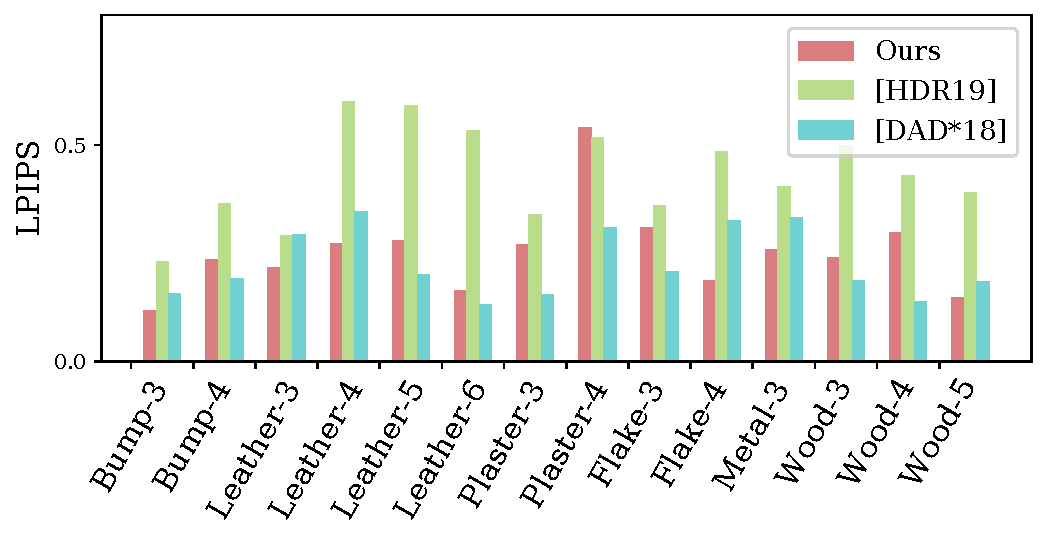
\includegraphics[width=0.8\columnwidth]{bayesian/fig7/LPIPS.pdf}
	\end{tabular}
	\caption[Quantitative evaluation]{\label{fig:bayesian:plot}
		\textbf{Quantitative evaluation.} The LPIPS of our results are consistently better than \cite{hu2019novel}. Some LPIPS values from \cite{deschaintre2018single} are better than ours, since (as per-pixel methods) they can better match the noise patterns in the textures.
	}
\end{figure}